
% !TEX encoding = latin1
% !TEX TS-program = pdflatex
% !TEX root = ../handout_qft.tex
% !TEX spellcheck = it-IT

%*******************************************************
% Chapter 1
%*******************************************************

\myChapter{Schwinger's own way to teach quantum mechanics}
%\myChapter{Schwinger's approach to quantum mechanics}
\label{chp:fundamentals} 

%\minitoc\mtcskip

\begin{refsection}
\begin{quoting}
   \openquote 
   I presume that all of you have already been exposed to some undergraduate
   course in Quantum Mechanics, one that leans heavily on de Broglie waves and
   the Schroedinger equation. I have never thought that this simple wave
   approach was acceptable as a general basis for the whole subject, and I
   intend to move immediately to replace it in your mind by a foundation that
   \emph{is} perfectly general.~\closequote
   \begin{flushright}
       J. Schwinger,
       \emph{Quantum Mechanics. Symbolism of Atomic Measurements}
       \textcite{Schwinger:2001}.
    \end{flushright}
\end{quoting}

\section{Introduction}

\lettrine{C}{ompared} 
to other areas of physics, quantum mechanics presents unique challenges.
On one hand, quantum theory stands as a great reminder of how intuition can be misleading and untrustworthy.
 Intuitions derived from classical physics often fall short in comprehending the behaviors of the quantum world.
  On the other hand, the mathematical machinery required to adeguately formulate quantum mechanics carries a substantial initial complexity, and it can obfuscate some of the physical implications, or at least it represents a technical distraction from the main area of focus. 

  One might wonder: is this level of mathematical sophistication required from the outset?
  As we will soon see, the inherent properties of quantum systems --- 
  such as Heisenberg's uncertanty principle, the intriguing role of probability in predicting the
outcomes of a quantum measurement, entanglement and superposition of quantum
  states --- demand richer mathematical abstractions capable of accommodating and
encoding such behaviors. 
  Classical formalism have proven inadeguate to 
describe such phenomena, naturally driving the necessity for alternative formulations.

Remarkably enough, quantum mechanics not only triggered a shift in perspective about physics itself, but also forced to expand the toolkit required to mathematically model


For example, incompatibility between physical measurable quantities like position and
momentum, which is at the root of uncetainty principle, can be described in
terms of \emph{non-commutative} objects, leading naturally to adopt matrices or
operators (instead of usual numbers) to describe position and momentum.
As we shall see, the canonical commutation relations imposed event further
requirements: they can't be realized in finite-dimensional vector spaces,
so we need to look at infinite-dimensional (Hilbert) spaces. 

Can we avoid Hilbert space?
As we shall see in the last part, other descriptions are possible, in
particular the path integral approach to quantum mechanics due to Feynman. 

In chapter~3, we will present and throughly discuss  all the postulates of  
non-relativistic quantum
mechanics. 
They have been distillized in the Twenties and Thirtees of '900 after  at least two
decades of strong and fashinating efforts, 
theoretical and experimental progress, wrong
attempts, mistakes, etc 
made by the intellectual fathers of quantum mechanics 
to eventually capture the essential  rules underlying 
the microscopic behavior of particles.

For example, consider classical electrodynamics. 
One can ask: are fields ``necessary''?


% Navigando a vista in un mare allora sconosciuto, inciampando negli
% imprevisti, 
% un percorso di intuizioni poi dimostratesi erronee, tentativi andati a vuoto
% vicoli ciechi, intuizioni che hanno spronato direzioni importanti per poi non
% trovare posto nella costruzione definitiva. 
% Questo lavoro e' confluito e si riassume nei postulati della meccanica
% quantistica.
% La loro validita' si poggia in ultima analisi sull'accordo con i fatti  sperimentali ovviamente, come per ogni
% branca della fisica. La loro forma e' quella a cui sono approdotati coloro
% che 
% Tuttavia, l'elevato livello di astrazione che li caratterizza, puo' 



\begin{figure}
   \centering
   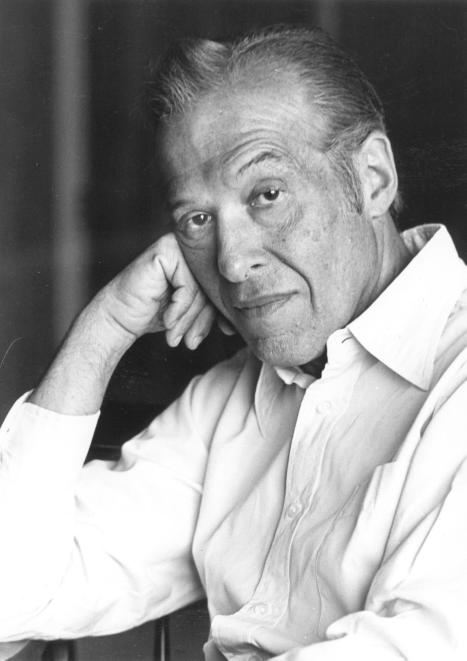
\includegraphics[scale=.35]{./Images/schwinger}
   \caption{Julian Seymour Schwinger (February 12, 1918 -- July 16, 1994) }
\end{figure}

\printbibliography[heading=subbibliography]
\end{refsection}
